\documentclass[12pt, oneside]{article} 
\usepackage{amsmath, amsthm, amssymb, calrsfs, wasysym, verbatim, bbm, color, graphics, geometry, multirow, booktabs}
\usepackage{graphicx}
\usepackage{tikz}
\usepackage{amsmath}
\usepackage{graphicx}
\usepackage{amsmath, amssymb, amsthm}
\usepackage{setspace}
\usepackage{tikz}
\usetikzlibrary{trees, positioning}
\usepackage{pgfplots}
\renewcommand{\baselinestretch}{1.0}
\geometry{tmargin=.75in, bmargin=.75in, lmargin=.75in, rmargin = .75in}  

\newcommand{\R}{\mathbb{R}}
\newcommand{\C}{\mathbb{C}}
\newcommand{\Z}{\mathbb{Z}}
\newcommand{\N}{\mathbb{N}}
\newcommand{\Q}{\mathbb{Q}}
\newcommand{\Cdot}{\boldsymbol{\cdot}}


\title{SP25 8732: Homework 2}
\author{Danbo CHEN}
\date{\today}

\begin{document}

\maketitle
\vspace{.25in}

\section{Question 1}
\textbf{Solution:}

\begin{center}
    
    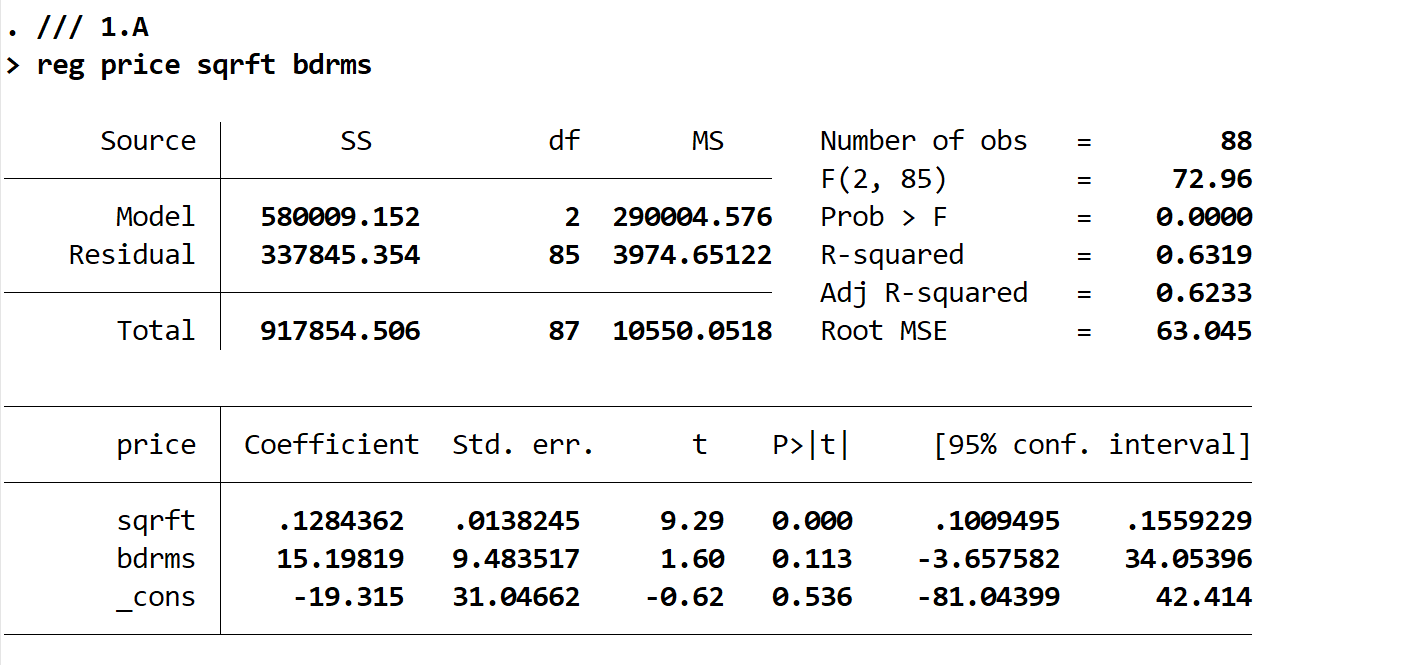
\includegraphics[width=0.8\textwidth]{Figure/P1.A.jpg}

    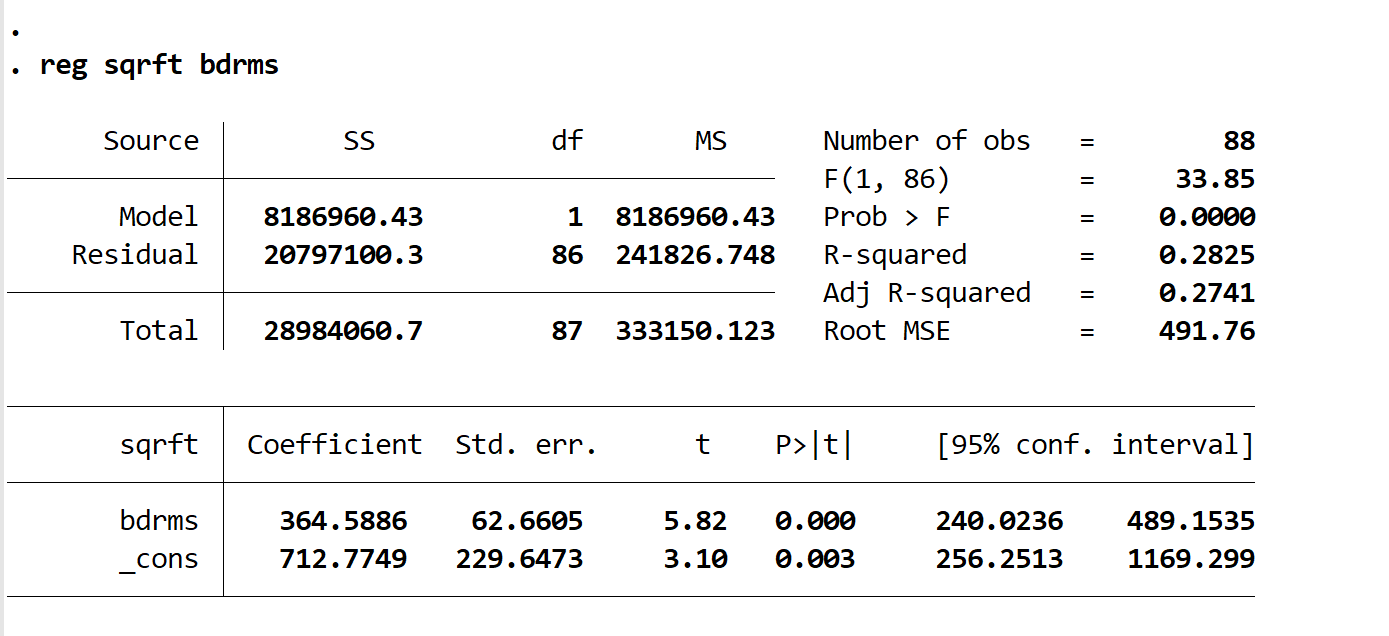
\includegraphics[width=0.8\textwidth]{Figure/P1.B.jpg}

    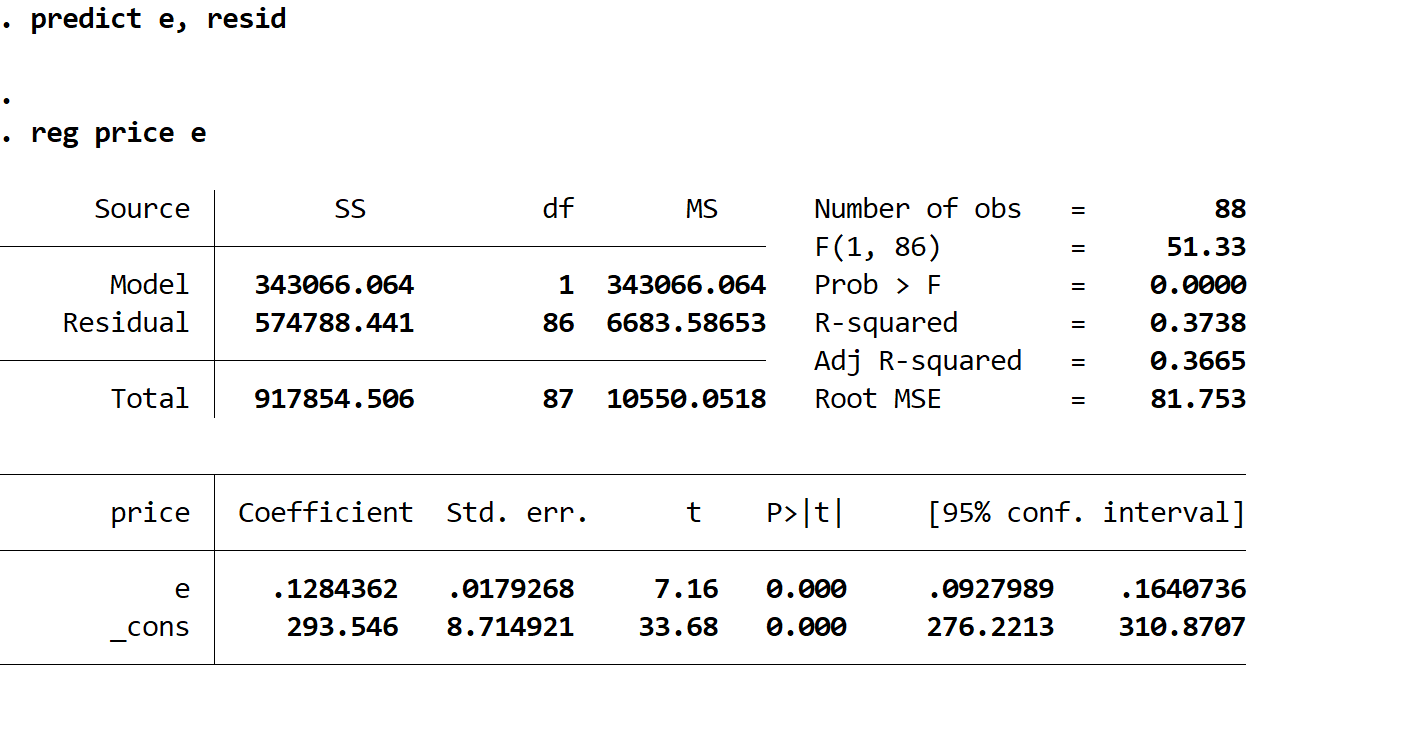
\includegraphics[width=0.8\textwidth]{Figure/P1.C.jpg}

\end{center}


\section{Question 2}
\textbf{Solution:}

\begin{center}

    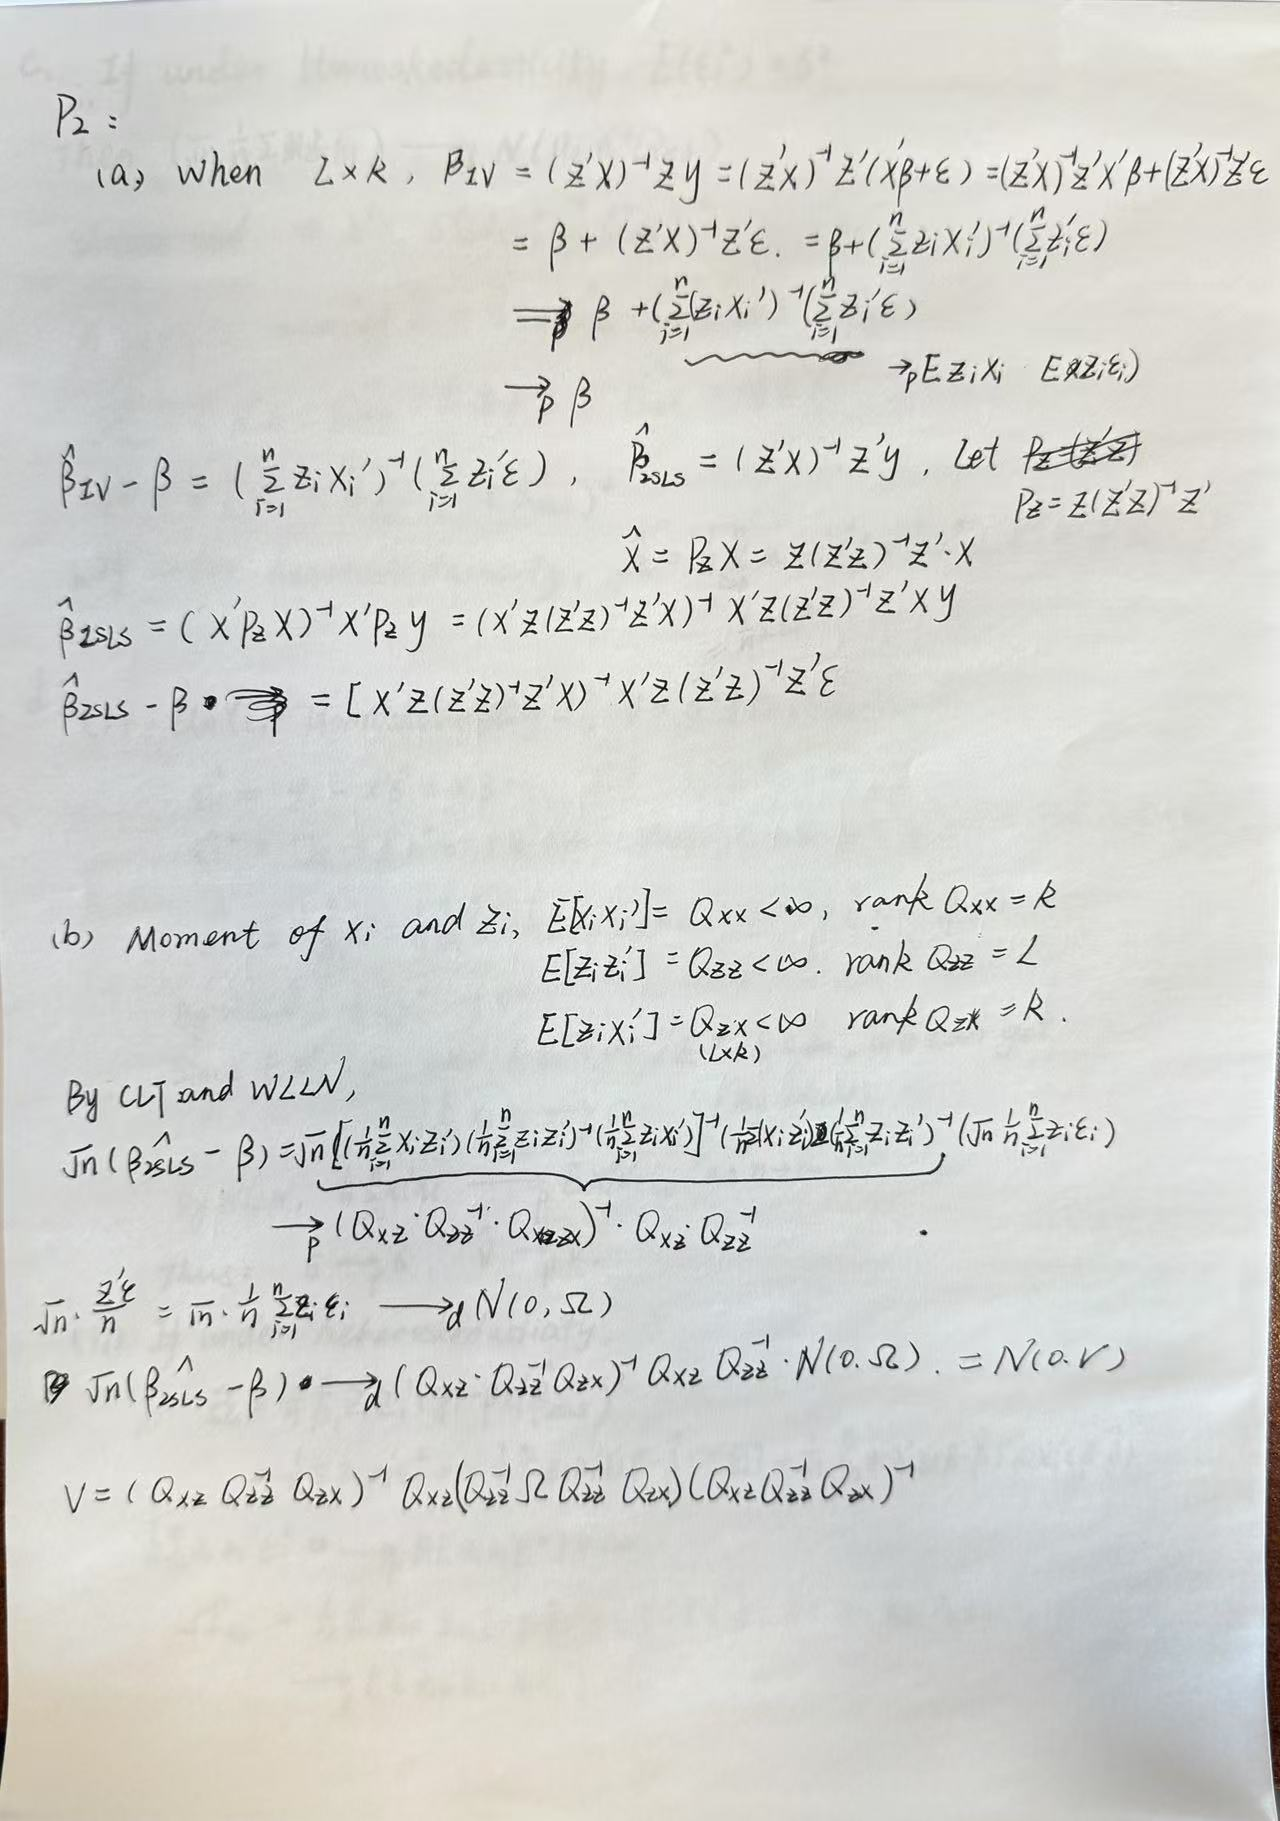
\includegraphics[width=0.8\textwidth]{Figure/P2.1.jpg}

    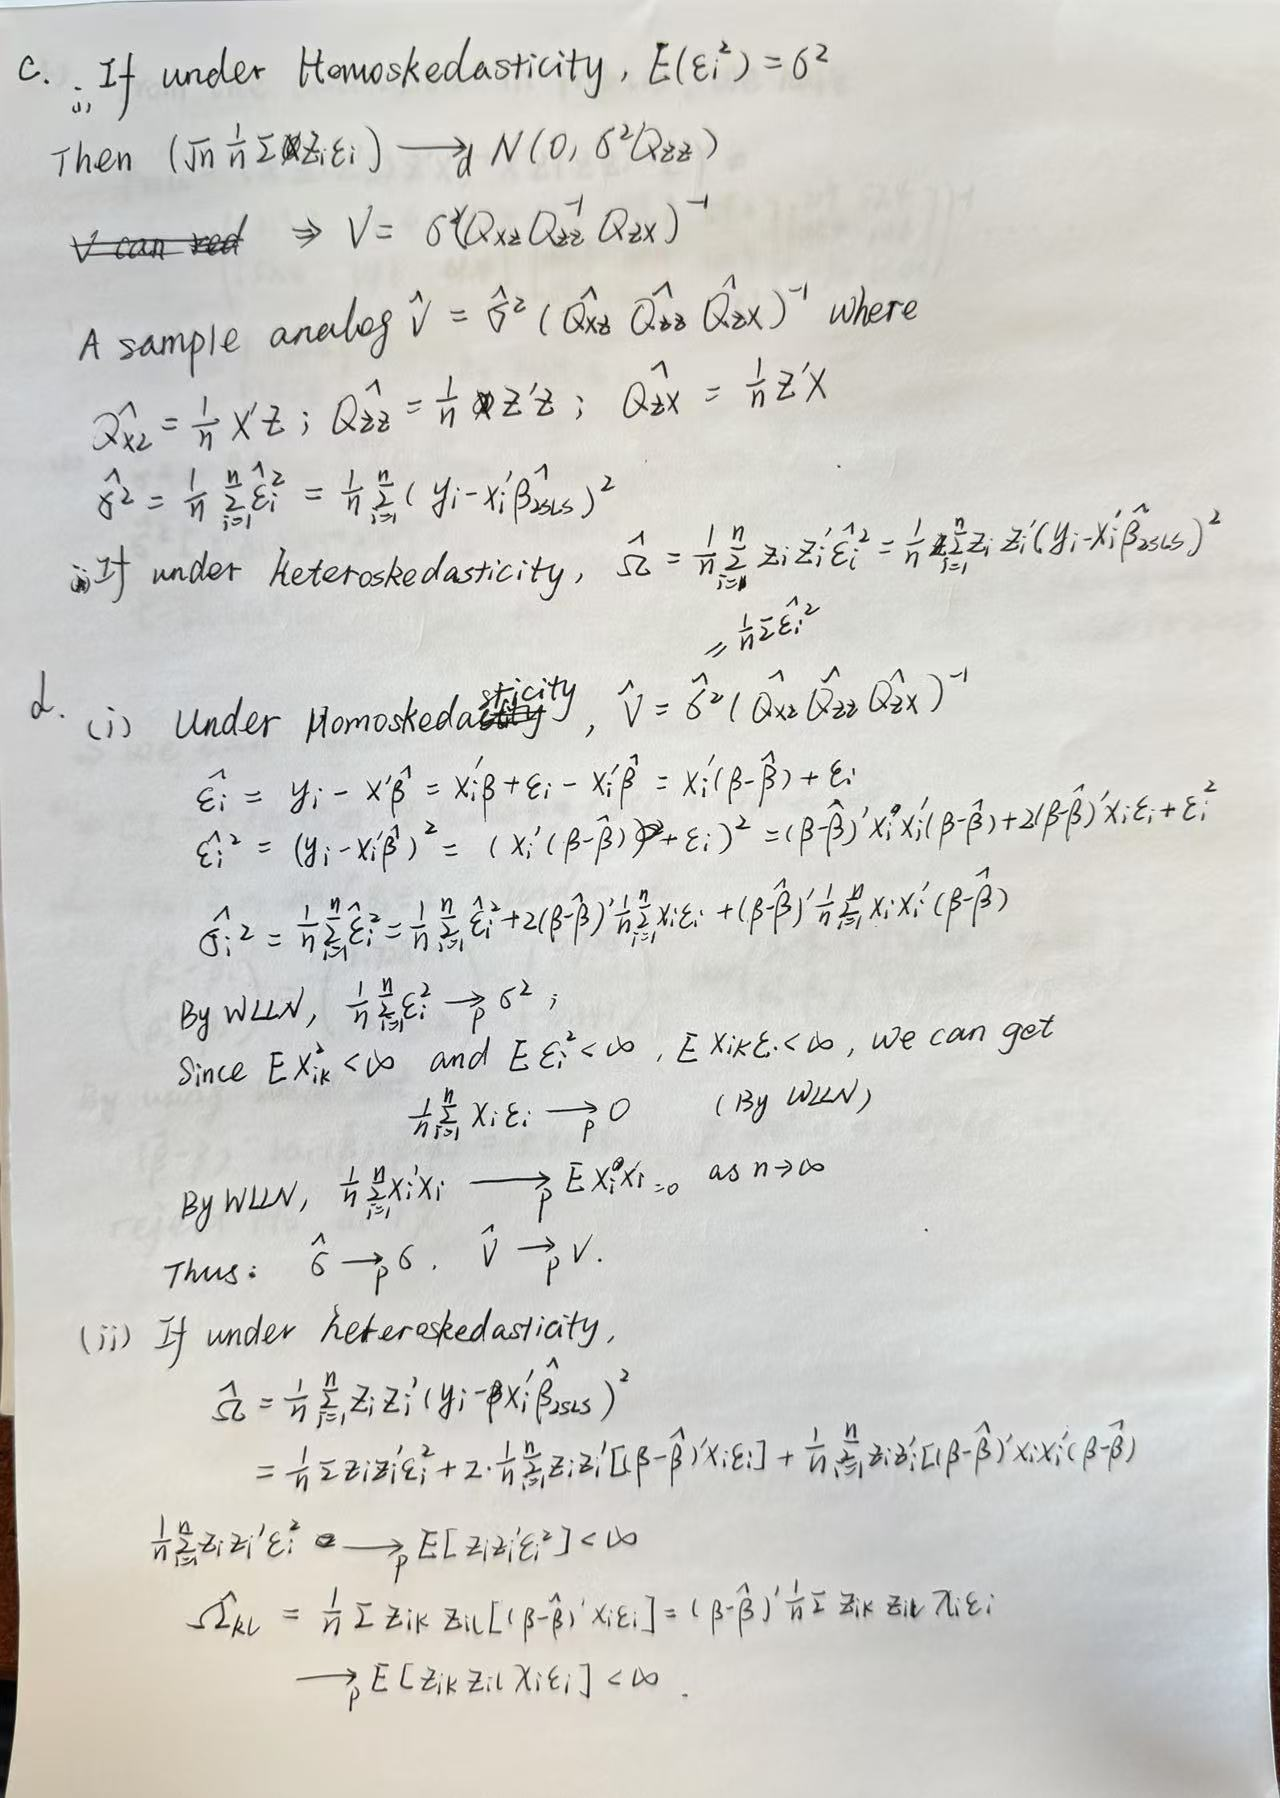
\includegraphics[width=0.8\textwidth]{Figure/P2.2.jpg}
\end{center}

\section{Question 3}
\textbf{Solution:}

\section{Question 4}
\textbf{Solution:}

\section{Question 5}
\textbf{Solution:}

\end{document}